
\documentclass[10pt,journal,compsoc]{IEEEtran}
\usepackage{listings}
\usepackage[pdftex]{graphicx}    
\usepackage{cite}

\usepackage{color}

\definecolor{mygreen}{rgb}{0,0.6,0}
\definecolor{mygray}{rgb}{0.5,0.5,0.5}
\definecolor{mymauve}{rgb}{0.58,0,0.82}

\lstset{ 
  backgroundcolor=\color{white},   % choose the background color; you must add \usepackage{color} or \usepackage{xcolor}; should come as last argument
  basicstyle=\footnotesize,        % the size of the fonts that are used for the code
  breakatwhitespace=false,         % sets if automatic breaks should only happen at whitespace
  breaklines=true,                 % sets automatic line breaking
  captionpos=b,                    % sets the caption-position to bottom
  commentstyle=\color{mygreen},    % comment style
  deletekeywords={...},            % if you want to delete keywords from the given language
  escapeinside={\%*}{*)},          % if you want to add LaTeX within your code
  extendedchars=true,              % lets you use non-ASCII characters; for 8-bits encodings only, does not work with UTF-8
  frame=single,	                   % adds a frame around the code
  keepspaces=true,                 % keeps spaces in text, useful for keeping indentation of code (possibly needs columns=flexible)
  keywordstyle=\color{blue},       % keyword style
  language=Octave,                 % the language of the code
  morekeywords={*,...},            % if you want to add more keywords to the set
  numbers=left,                    % where to put the line-numbers; possible values are (none, left, right)
  numbersep=5pt,                   % how far the line-numbers are from the code
  numberstyle=\tiny\color{mygray}, % the style that is used for the line-numbers
  rulecolor=\color{black},         % if not set, the frame-color may be changed on line-breaks within not-black text (e.g. comments (green here))
  showspaces=false,                % show spaces everywhere adding particular underscores; it overrides 'showstringspaces'
  showstringspaces=false,          % underline spaces within strings only
  showtabs=false,                  % show tabs within strings adding particular underscores
  stepnumber=2,                    % the step between two line-numbers. If it's 1, each line will be numbered
  stringstyle=\color{mymauve},     % string literal style
  tabsize=2,	                   % sets default tabsize to 2 spaces
  title=\lstname                   % show the filename of files included with \lstinputlisting; also try caption instead of title
}

\hyphenation{op-tical net-works semi-conduc-tor}


\begin{document}

\title{Realsense2 RTABMAP}

\author{Jung, Myoungki}

\markboth{SLAM project, Robotics Nanodegree Program, Udacity}%
{}
\IEEEtitleabstractindextext{%

\begin{abstract}
A simultaneous localisation and mapping(SLAM) has been a classic complex problem topic in therobotics field. Realtime apperance based mapping (RTABMAP) package shows its approach to tackle down the using the data from vision based sensors.
The purpose of this report is to show the application of off the shelf localisation package inin a simulated condition, robotics operating system(ROS), its implementation, tunning parameters and results.
\end{abstract}

% Note that keywords are not normally used for peerreview papers.
\begin{IEEEkeywords}
Robot, IEEEtran, Udacity, ROS, RTABMAP, SLAM.
\end{IEEEkeywords}}

\maketitle
\IEEEdisplaynontitleabstractindextext
\IEEEpeerreviewmaketitle
\section{Introduction}
\label{sec:introduction}

\IEEEPARstart{2}{W1H} , when and where and how, is the main compoment of a task for any job delegated agents, humans as well as robots. The topic solving the where the agent is simultaneous localisation and mapping. SLAM is an essential tool for discovering never visited area, or continously changing working area.

\section{Background}
Classic SLAM algorithm has been evolved to many variations. However, Grapsh SLAM was used as its accuracy and capability, also adavantages over other modern SLAM algorithms.

\begin{figure}[thpb]
      \centering
      \includegraphics[width=\linewidth]{./img/CSLAM.jpg}
      \caption{Category of SLAM}
      \label{fig:CSLAM}
      \cite{Thrun2002}
\end{figure}

Figure \ref{fig:CSLAM} shows the category of SLAM algorithms.

\subsection{Fast SLAM}
Fast SLAM is a full and online slam which uses monte carlo localisation(MCL) + Low-Dimensional EKF to solve SLAM problem. Its version 1.0 and 2.0 both also low dimensional extended kalman filter. Version 2.0 is more efficient than the version 1.0 by using different distribution with a low number of particles than the predecessor. 
Figure \ref{fig:FastSLAM} shows the relation of fast SLAM category. The Grid based FastSLAM is an extension of FastSLAM using grid maps and this SLAM offers non landmark based SLAM by using MCL, for sample motion and importance weight, and occupancy grid mapping for map estimation.

\begin{figure}[thpb]
      \centering
      \includegraphics[width=\linewidth]{./img/FastSLAM.png}
      \caption{Category of SLAM}
      \label{fig:FastSLAM}
      \cite{Thrun2002}
\end{figure}


\subsection{Grapsh SLAM}
Graph SLAM can solve a full SLAM, covering the entire path and map. The SLAM is consist of Two Tasks, Front-end and Back-end. Algorithm constructs the graph using the odometery and sensory measurements collected by the robot in the Front-end. he Back-end task optimizes the graph. Maximum Likelihood Estimation(MLE) performs the graph optimization by applying an optimization algorithm such as stocastic gradient descent.

\subsection{Real Time Appearance Based Mapping (RTABMAP)}
RTABMAP is an open source library implementing loop closure detection with a memory management approach to support online requirements for long-term and large-scale environment mapping\cite{Labbe2018}.
Infolab of RTAB-Map published a cross-platform standalone C++ library and a ROS package. Inputs from scanner data to visual images are processed by RTAB MAP and results a map (2D or 3D) and optionally occupancy grid, point clouds.

\section{Scene and robot configuration}
\subsection{Robot}
The agent model, shown in Figure \ref{fig:racersupportarmd435}, is a slight modified version of previous localisation model, racerbot, with an heightened camera support on the chassis.

\begin{figure}[thpb]
      \centering
      \includegraphics[width=.5\linewidth]{./img/racersupportarmd435.png}
      \caption{Agent model}
      \label{fig:racersupportarmd435}
\end{figure}

\subsection{Sensors}
The only visual sensor, realsense D435 plugin was used and hokyuo scanner was not used but not removed. Due to usage of d435, hokyuo's scan data was replaced by the \verb!depth_registered/points! topic from the intel D435 RGBD camera.
The used sensors are shown in Table \ref{table:model_design}.
\begin{table}[ht]
      \caption{Model Design}
      \label{table:model_design}
      \begin{center}
      \begin{tabular}{|c|c|}
      \hline
      Atribute & Value \\
      \hline\hline
      Agent & 0.15 m by 0.10 m \\
      \hline
      Camera & RealSense D435 \\
      \hline
      Scanner & hokyuo \\
      \hline
      \end{tabular}
      \end{center}
\end{table}

\subsection{Packages}

The list below contains the packages used in this project
\begin{enumerate}
      \item \verb!Move_base!
      \item \verb!RTABMAP_ros!
      \item \verb!RealSense!
      \item \verb!standalone_nodelet! for converting mm to m and Depth to \verb!depth_registered/points!
      \item teleop package
\end{enumerate}
Lauch files, \verb!world.launch! and \verb!mapping.launch! creates the package layout shown in Figure \ref{fig:rqtrosgraph}. \verb!move_base! and \verb!amcl! also were used for SLAM in ROS. However, \verb!amcl! is not a neccessary package for localisation as rtabmap provides localisation mode too.

\begin{figure}[thpb]
      \centering
      \includegraphics[width=\columnwidth]{./img/rqtrosgraph.png}
      \caption{rqtrosgraph view}
      \label{fig:rqtrosgraph}
\end{figure}

\subsection{Launch Process}
The List \ref{list:RTABMAPMappinglaunch} shows how to start mapping. The previous data base of rtabmap is erased when mapping starts. The mapping by teleop package is shown in Figure \ref{fig:rtabmapmappingprocess}. Mapping can be done with rviz by assigning goal pose. However, the move package can maneuver in unexpected ways and corrupt the entire map easily.
\begin{lstlisting}[language=sh, caption={RTABMAP mapping launch command},label={list:RTABMAPMappinglaunch}]
$ roslaunch slam_project world.launch
$ roslaunch slam_project mapping.launch rtabmap_args:="--delete_db_on_start" rtabmapviz:=false rviz:=true
$ roslaunch slam_project teleop
\end{lstlisting}

The difference from the original mapping parameters from the provided files from udacity is listed on The Listing \ref{list:RTABMAPMappingDiff}. The occupancy grid map easily duplicated features and corrupted the integrity of the grid map. Therefore the limits for 'LinearSpeedUpdate' and 'AngularSpeedUpdate' was set to remove the corrupting artifacts while moving slower than 0.2 m/s or 0.2 rad/s. I addition, the RGBD camera's `MaxDepth` was limited to 3.5 m as more than this range is very noisy.
\begin{lstlisting}[language=XML, caption={Diff RTABMAP mapping.launch},label={list:RTABMAPMappingDiff}]
<param name="RGBD/LinearSpeedUpdate" type="string"  value="0.1"/>
<param name="RGBD/AngularSpeedUpdate" type="string"  value="0.1"/>
<param name="RGBD/LoopClosureReextractFeatures" type="string"  value="true"/>

<param name="RGBD/ProximityBySpace" type="string"  value="true"/>

<param name="Kp/MaxDepth" type="string"  value="3.5"/>  
\end{lstlisting}

\begin{figure}[thpb]
      \centering
      \includegraphics[width=\columnwidth]{./img/rtabmapmappingprocess.png}
      \caption{Rtabmap mapping process}
      \label{fig:rtabmapmappingprocess}
\end{figure}

The listing \ref{list:RTABMAPMappinglaunch} shows code enabling localisation from the existing map from the mapping process.
In localisation mode, the working memory is initialised with the provious map data and does not overwrite on it during robots' navigation. localisation was tested by moving robot randomly and start the localisation mode.

\begin{lstlisting}[language=XML, caption={Diff RTABMAP localisation.launch},label={list:RTABMAPLaunchDiff}]
<param name="Mem/IncrementalMemory" type="string" value="false"/>
<param name="Mem/InitWMWithAllNodes" type="string" value="true"/>
\end{lstlisting}

\begin{lstlisting}[language=sh, caption={RTABMAP localisation launch command},label={list:RTABMAPlocalisationlaunch}]
$ roslaunch slam_project world.launch
$ roslaunch slam_project mapping.launch rtabmapviz:=false rviz:=true
\end{lstlisting}

The shell commands in List \ref{list:RTABMAPMappinglaunch} starts localisation mode shown on Figure \ref{fig:localisationprocess}.
\begin{figure}[thpb]
      \centering
      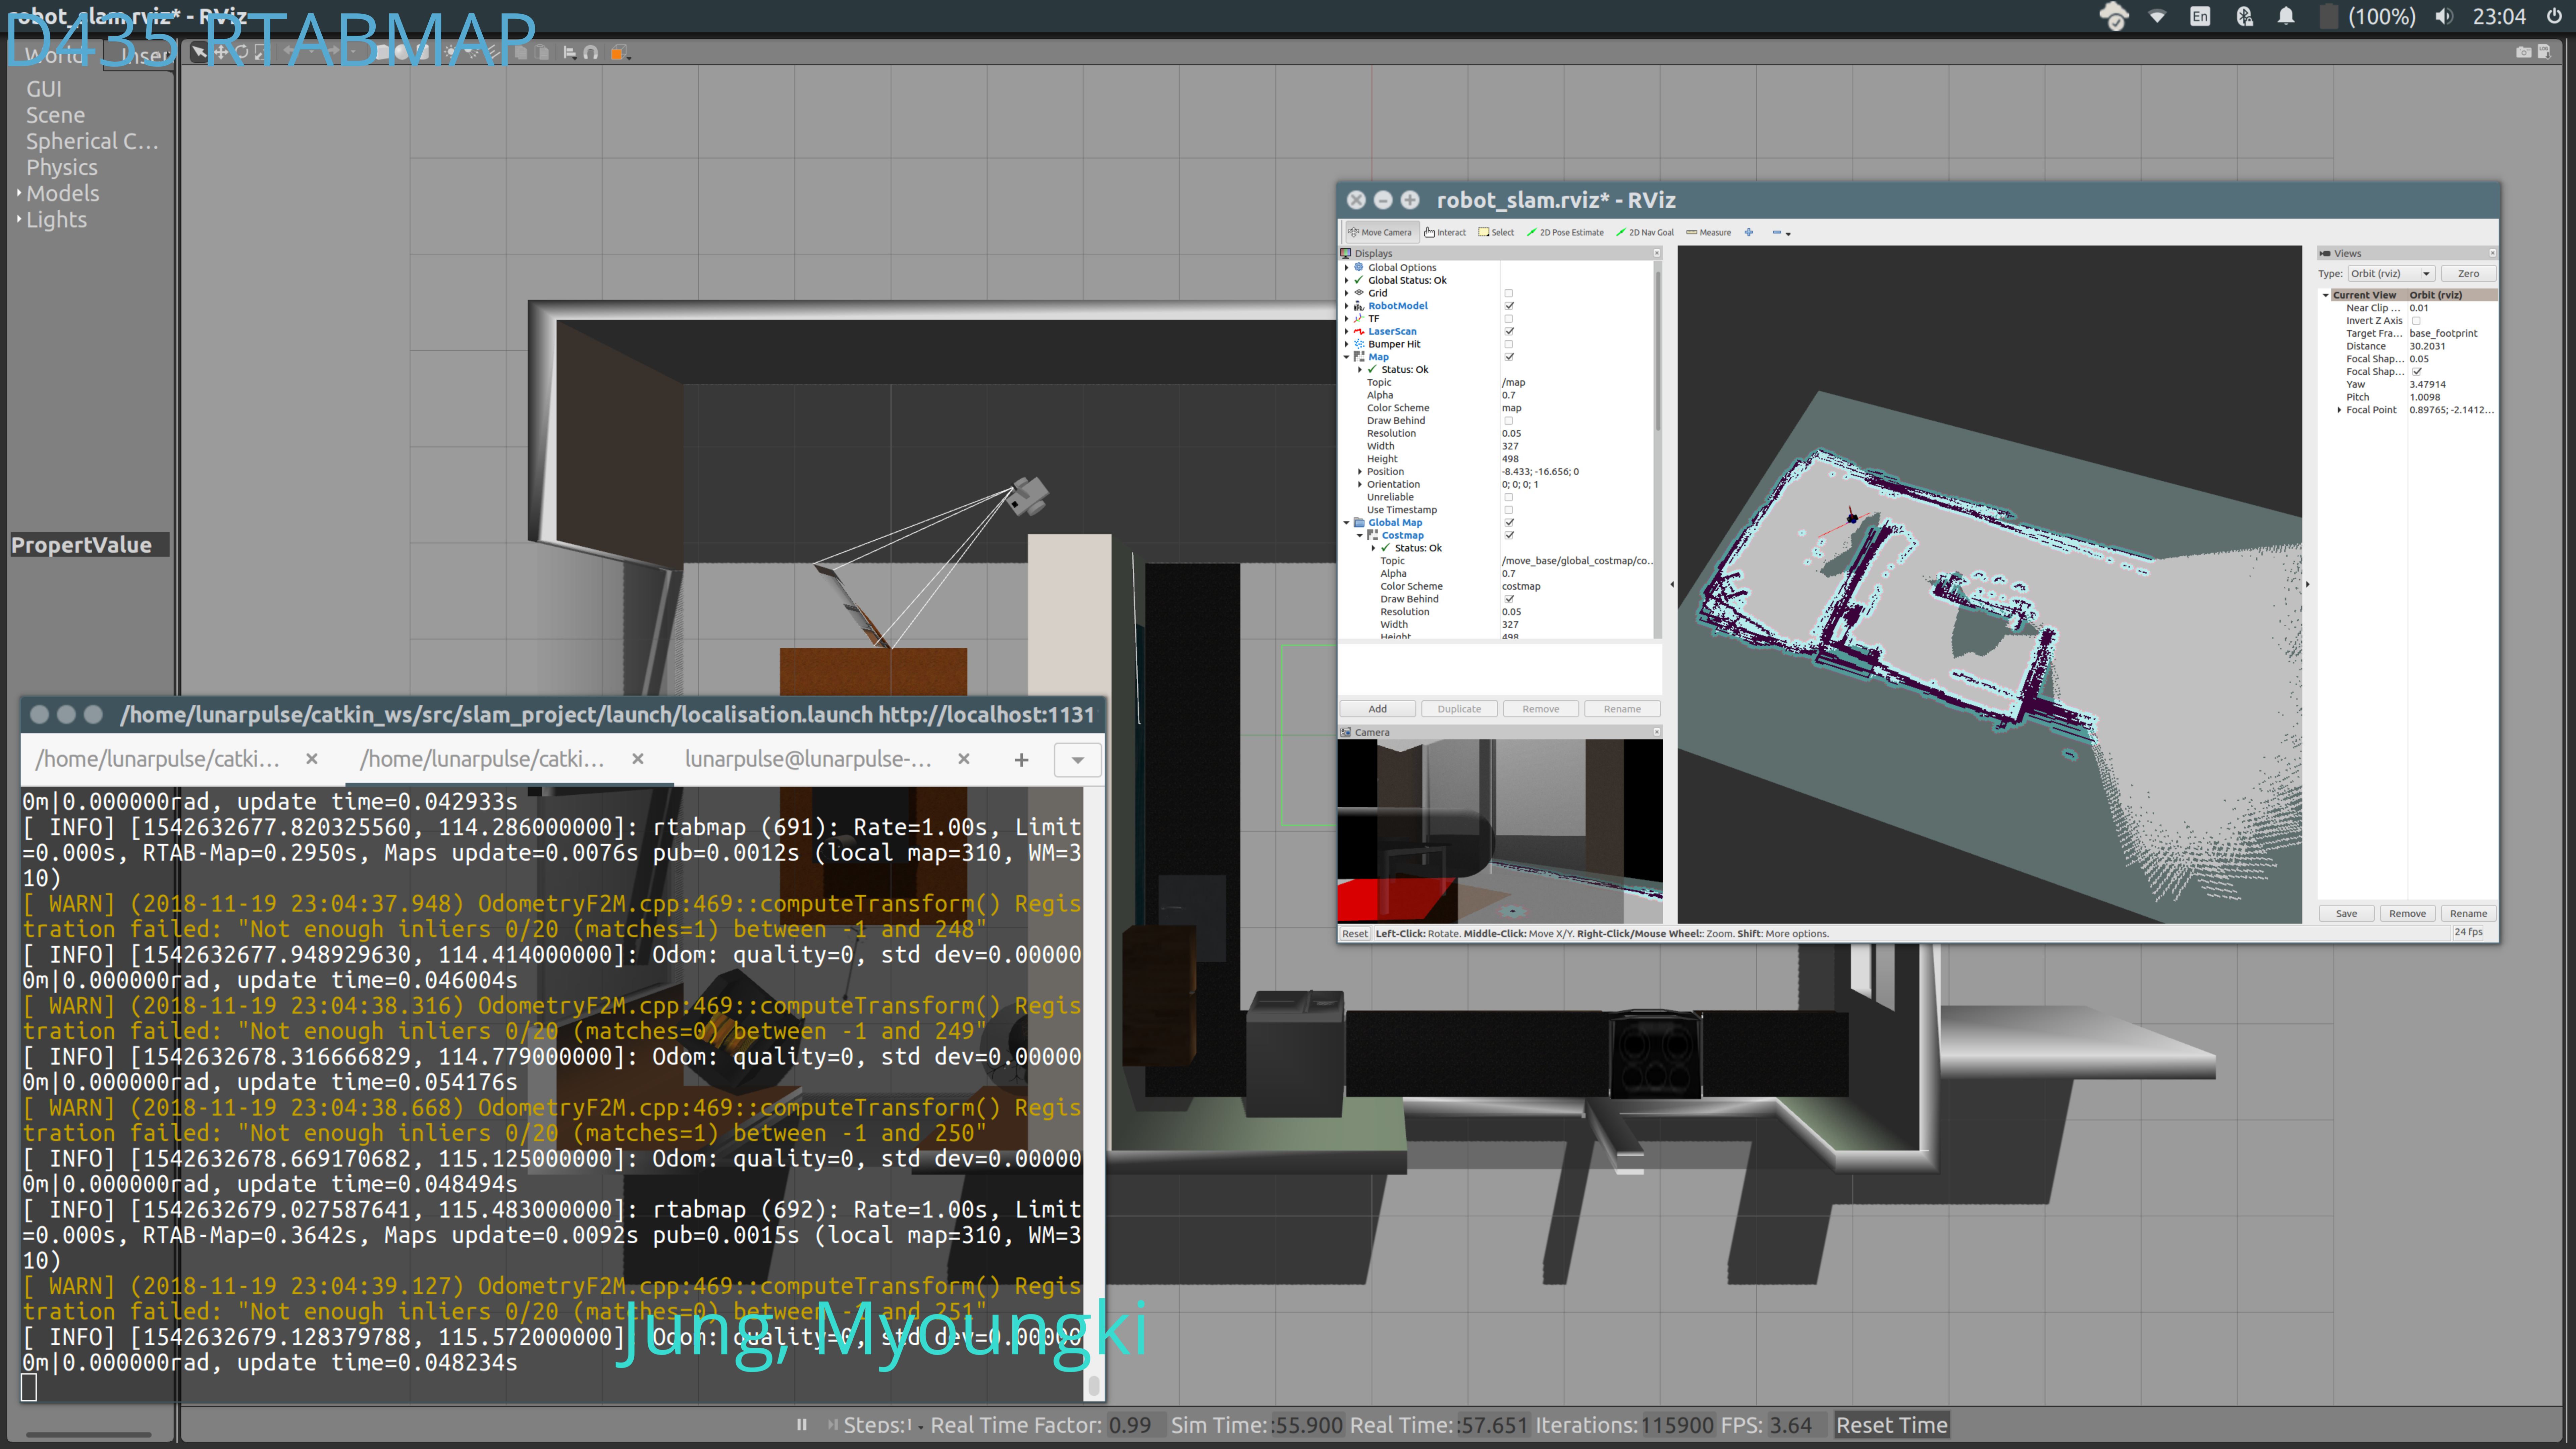
\includegraphics[width=\columnwidth]{./img/localisationprocess.png}
      \caption{Rtabmap localisation process}
      \label{fig:localisationprocess}
\end{figure}

\section{Results}
\subsection{Benchmark scene - Kitchen and Dining}
The benchmark world kitchen and dining imposed some difficulty in creation of occupancy grid mapping. The turning velocity had to be very slow. With the provided teleop package, a stasfactory level of details in mapping could be acheived.
The result of mapping process in kitchen and dining world in rtabmap database viewer is shown on Figure \ref{fig:kdrtabmapdbview}. The number of loop closure is 46 and has total 309 local map. The features in the scene, chairs, tables, lamp, sofa, and etc. can be recognisable from the occupancy grid map. The map view shows clear single lined walls of the building. If it was normal \verb!kinect!, instead of \verb!realsense_gazebo_plugin!, it could be easier to acheive cleaner map and occupancy grid map. The \verb!realsense_gazebo_plugin! used for this project has flaws and instability, resulting jumps in odometery, excessively slow in complex scene.
\begin{figure}[thpb]
      \centering
      \includegraphics[width=\linewidth]{./img/kdrtabmapdbview.png}
      \caption{kitchen and dining rtabmap data base view}
      \label{fig:kdrtabmapdbview}
\end{figure}
The challenge of mapping was how patiently move and planning before moving the agent. Localisation was successful, Figure \ref{fig:localisationprocess}, even with kidnapped robot scenario and this shows the strength of rtabmap.

\subsection{My model - gazebo}

\verb!/world/gazebo.world! contains second custom world file for this project, \verb!gazbo.world!. The  \verb!gazbo.world! has rich visual features, due to the trees, and makes it easier to SLAM compared to the benchmark kitchen and dining world. However, processing of tree branches and leaved slows down the overall ROS system occationally. The result of mapping process in this scene was saved in . Figure \ref{fig:gazebo_rtabmapdbview} shows the rtabmap databse view of the mapping result in gazebo world. The details of objects in the scene are cleary shown, SUV, walking person, can, rag doll, gazebo, fountain and the exact number of trees. Mapping in this world was done by rviz and performed SLAM instead of mapping. The agent was able to map the new environment and localise itself inside it using the obtained map. The number of loop clousure is 7 and it was intentinally avoided to have too many loop closures by not visiting the same place many times to avoid the creation of duplicated features in occupancy grid map.
\begin{figure}[thpb]
      \centering
      \includegraphics[width=\linewidth]{./img/gazebo_rtabmapdbview.png}
      \caption{gazebo rtabmap data base view}
      \label{fig:gazebo_rtabmapdbview}
\end{figure}

In both scenarios, loop closures were observed in rviz. The map data shown in rviz wes updated and this shows \verb!map data! of rtab was updated prior to rviz.
THe dababase files are bigger than normal created by kinect sensors, as the size of scan data from d435 is much larger than the one by hokyuo and this larger scan data makes SLAM dababase bigger.
\section{Discussion}
 
The tuning process of the SLAM was non-trivial task and requires understanding of many parameters, the incomplete and unstable \verb!realsense_gazebo_plugin! added more difficulty. The implication of loop closure for healing every problem in mapping should be discarded. The mapping must be carefully done but not expecting loop closure function to fix poor mapping process. The loop closure should be only used to recover from disrupted map due to the mapping errors, odometry drift, IMU drifts, sensor noises. In other words, speedy mapping required by fast autonomous vehicles, drones, uav, ugv, and autonomous flying cars, is far from the current technology and this has be be solved for the required technology.

\section{Conclusion / Future work}
The RTABMAP tends to create a displaced occupancy grid map and persists the wrong artifacts for long time. Once this happens, an agent need to map from the beginning again. There might be parameters prevent this happening or allow less occurences, the documentation on RTABMAP is not sufficent to find it easy. RTABMAP should take this to be accounted and make the parameter tuning more straight fowards for the users' precious time and effort.
RGBD still contains much errors in output point clouds. And this propagates to the final SLAM result. RTABMAP is just as good as collision avoidance level accuracy not for fine maneuver purposes.

Drones can construct 3D maps of the rescue mission in dangerous area, such disaster zone, underground working area, radio activity infuenced area. However, the zone specific challenges exists, visibility for visual odometery, richness of textures also affects the choice of slam, RTABMAP can only be used in optimal visual condition filled with rich texturised objects. This can be still used with a good environment conditioning, sufficient ambient lights and clear atmosphere but not for heavy industrial, dusty and monotonous area. From these limitation of visual based mapping, home service unit can be suited best.
Another one noticeable is that RTABMAP uses SURF or SIFT, visual feature matching algorithms. With the recent progress in machine learning, especially neural networks, those image reocognition methods can be replaced with well trained CNN or voxnet, 3d volumetric convolutional neural network \cite{Maturana2015c} for specific envrionment to improve accuracy and range of the feature recognition. In addition, deep reinforcment learning can be a good candidate for new SLAM approach.

\bibliography{bib}
\bibliographystyle{ieeetr}

\end{document}
